\section{Genetic algorithm}
Genetic algorithms are based on the idea of evolution, that the most suited individuals tend to live longer and reproduce. 
\subsection{Description}
In Genetic Algorithms, or GAs, a population is simulated in an artificial world using a combination of reproduction, gene crossover and mutation, with a given goal for the population to achieve.\cite{GAHandbook1}\\
\\
Due to the need to simulate the population and evaluate individuals, often multiple times, GAs are not well suited for all kind of problems. When there exists an analytical solution it may be better to use that. However, if the problem can be simulated, both problems without analytical solutions and problem with complicated analytical solutions can be handled by GAs, although it is never guaranteed to give an optimal solution.\\
\\
As in nature, a population consisting of individuals are used. Each individual has one or more chromosomes, each with one or more genes. During each generation, individuals are selected and paired for reproduction, often with higher selection pressure on more fit individuals, and their genes are combined to form new children. Also, as in the real world, mutations can occur.\\
\\
%% Generational / Steady-state
GAs can either be steady-state or generational, where steady-state means that the current population is altered, and generational is when a new generation is created and replaces the old.\\
\\ 
%% Pseudo-code
\\Pseudo-code for Genetic Algorithm:
\begin{enumerate}
\item Start with an initial population
\item Select parents for reproduction
\subitem Perform crossover
\subitem Do mutation
\subitem Replace parents in new generation
\item Repeat from step 2
\end{enumerate}
\begin{figure}[hb]
  \centering
  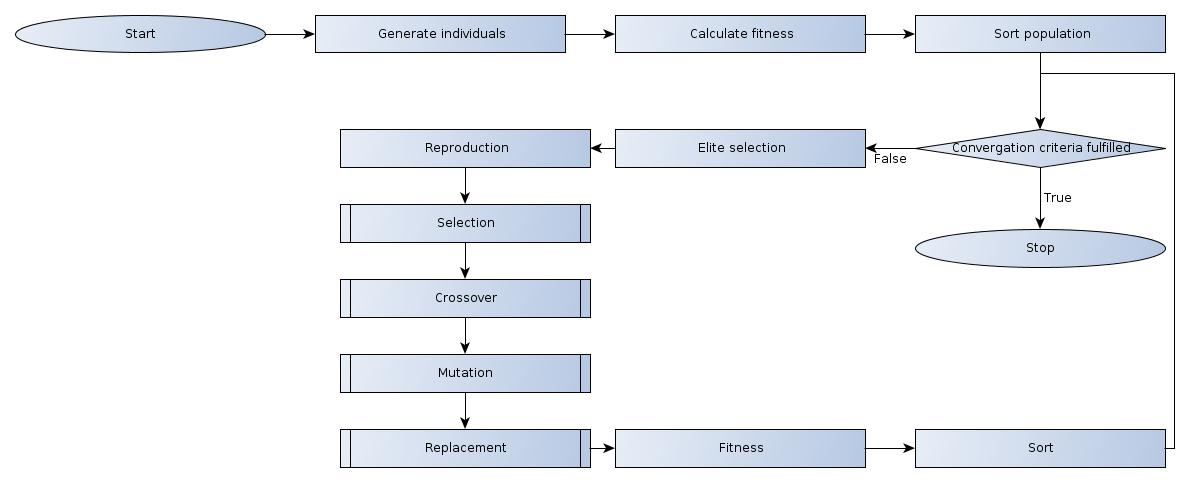
\includegraphics[width=6in]{chapter_4_methods/GeneticFlowChart.jpg}
  \caption[Flow chart of genetic algorithm]%
  {Flow chart of genetic algorithm}
\end{figure}
%% Selection (parents)
There are several ways to choose parents, but four methods are Fitness Proportionate Selection, Random Selection, Fit-Fit and Fit-Weak. In Fitness Proportionate Selection the probability of choosing a more fit individual is higher than to select a less fit individual. Roulette selection is one common method of selection that fits under this category. Random selection is another method, in which the probability to choose a certain individual is equal for all individuals.\\
%% Mutation
\\Mutation is important in GAs since it makes sure that all the search space can be reached, even if the initial population did not cover all of it.\\
%% Crossover
\\There are different methods for crossover, a few of those are n-point shuffle crossover, uniform crossover and variable crossover.\\
%% Replacement
\\When reproduction has been completed, in order to not increase the population size, a replacement has to be performed. For this there are several methods, such as Weak Parent, Both Parents, Weakest Individual and Random.\\
In Weak Parent, a weaker parent is replaced by a stronger child.\\
In Both Parents, the child replaces the parent.\\
In Weakest Individual, the children replaces the two weakest individuals in the population, if the children are fitter.\\
In Random, the children replaces random individuals in the population.\\
%% Termination
\\To make sure the algorithm ends at some point, a termination condition has to be used. It can be a maximum number of generations, a limit in fitness sum, a median fitness, best individual or worst individual.\\
With Fitness sum, the algorithm will terminate when the sum of the fitness for the population is less than or equal to a specified value.\\
With Median fitness, a range for the fitness is specified.\\
With best individual, the algorithm will terminate when the minimum fitness drops below a convergence value and thereby guarantee at least one good solution while saving time.\\
With Worst Individual, the algorithm will terminate when all individuals in the population has a fitness value lower than the convergence value.\\
\subsection{Development process}
How the development of the algorithm have proceeded.\\
%%\\
%%Parameters was set according to:\\
%%Cromosome length was set to \begin{math}n^2\end{math}, to be able to cover the entire environment.\\
%%Population size was set to ..., using 10.1.1.105.2431 "Optimal Population Size and the Genetic Algorithm".\\
%%Instance size was set to ...\\
%%Number of generations was set to ...\\

\subsection{Algorithm}
The algorithm consists of four parts, first an initial set of genes for each pursuer is generated and combined to form individuals in the population. When an initial population has been generated, the following is repeated until either a maximum number of generations has been reached or a the population has converged to a solution:\\
\begin{itemize}
\item Initial population
\item Reproduction%%, also called crossover. By using a selection method two individuals are selected to be parents for two children. Each child gets it's genes alternating from each parent, the first child gets the first gene from the first parent, the second from the second parent, the third from the first parent and so on. The second child gets the first gene from the second parent, the second gene from the first parent, and so on. For each child, there is a chance of mutation.
\item Crossover
\item Mutation.%% To make sure there can be variations in the population, mutations are used. It is important not to use mutations to often, since that can lead to a random approach instead. For each new child that is created, there is a possibility that a gene gets manipulated during the crossover. If this happens, the gene gets cut of at a random point, and that part is replaced by a new randomly generated sequence.
\item Selection. %%To make sure that the population will not grow indefinitely, a selection scheme is used. At each crossover there are four different individuals, two parents and two children. Selection is made by always keeping the two most fit individuals, which can either be children or parents.

\end{itemize}
During reproduction, which is also called crossover, new individuals are created to form a new population. First a selection procedure is preformed, in which 
%%Selection: A combination of elitism and random selection was used. Elitism to make sure good solutions was not lost, by always keeping all feasible solutions that solved the pursuit-evasion problem, and random selection to maintain a diversity.\\
%%Crossover: \\
%%Mutation: To make sure that all solutions can be obtained, mutations is used. However, to make sure that it will not only be a random search, the chance of mutation was 1% at crossover and 0% in all other cases.\\

\subsection{Implementation}
The algorithm is implemented using C. Previous written libraries for Genetic Algorithm was used as a reference, e.g. LibGA.

